\chapter{Atomic Orbitals: Shapes, Energies and Sizes}\label{ch:b2:atomic-orbitals}

A hydrogen atom has no edge: its electron may be found at any distance from
the nucleus, with a probability that falls off quickly but never reaches
zero. Yet atoms have sizes, and a sodium atom is about twice as wide as a
chlorine atom, though it holds fewer electrons. The Year 1 volume named the
states of an electron by three quantum numbers; here each of them becomes a
function of position, with a shape, nodes, signs and a size, and a simple set
of rules turns them into orbital energies for any atom. These shapes and signs
are what the next four chapters combine into molecular orbitals.

\begin{recall}
The Year 1 volume: quantum numbers $n$, $l$, $m_l$, $m_s$; atomic orbitals as the
states $(n, l, m_l)$; shells and subshells; screening and effective nuclear
charge (qualitatively); electron configurations; the levels of hydrogen,
$-E_R/n^2$ with $E_R = \qty{13.6}{eV}$. From physics: the \omterm{def:b2:atomic-orbitals:wavefunction}{wavefunction}, whose
squared modulus is a \omterm{def:b2:atomic-orbitals:wavefunction}{probability density}.
\end{recall}

\section{The wavefunctions of the hydrogen atom}

\begin{definition}[Wavefunction]\label{def:b2:atomic-orbitals:wavefunction}
The state of an electron is described by a \emph{wavefunction}\index{wavefunction}
$\psi(x, y, z)$; $|\psi|^2$ is its \emph{probability density}\index{probability
density}: the probability of finding the electron in a small volume $dV$ around
a point is $|\psi|^2\,dV$, and $\int|\psi|^2\,dV = 1$ over all space (the function
is normalised). An atomic orbital is the wavefunction of one electron in an
atom.
\end{definition}

\begin{definition}[Radial and angular parts]\label{def:b2:atomic-orbitals:radial-angular}
In spherical coordinates $(r, \theta, \varphi)$ about the nucleus, the orbitals of
a hydrogen-like atom factorise as $\psi_{nlm}(r, \theta, \varphi) = R_{nl}(r)\,
Y_{lm}(\theta, \varphi)$: the \emph{radial part}\index{radial part} $R_{nl}$ depends
on $n$ and $l$, the \emph{angular part}\index{angular part} $Y_{lm}$ on $l$ and
$m_l$ only.
\end{definition}

\begin{theorem}[The hydrogen-like orbitals]\label{thm:b2:atomic-orbitals:hydrogen}
For a one-electron atom of nuclear charge $Ze$, with $\rho = Zr/a_0$ and $a_0 =
\qty{52.9}{pm}$ the Bohr radius, the \omterm{def:b2:atomic-orbitals:radial-angular}{radial parts} for $n \leq 3$ are, in units of
$(Z/a_0)^{3/2}$:
\[
\begin{array}{ll}
  R_{1s} = 2\,\mathrm e^{-\rho} &
  R_{2s} = \dfrac{1}{2\sqrt2}\,(2 - \rho)\,\mathrm e^{-\rho/2} \\[2ex]
  R_{2p} = \dfrac{1}{2\sqrt6}\,\rho\,\mathrm e^{-\rho/2} &
  R_{3s} = \dfrac{2}{81\sqrt3}\,(27 - 18\rho + 2\rho^2)\,\mathrm e^{-\rho/3} \\[2ex]
  R_{3p} = \dfrac{4}{81\sqrt6}\,(6\rho - \rho^2)\,\mathrm e^{-\rho/3} &
  R_{3d} = \dfrac{4}{81\sqrt{30}}\,\rho^2\,\mathrm e^{-\rho/3}
\end{array}
\]
and the real \omterm{def:b2:atomic-orbitals:radial-angular}{angular parts} are $Y_s = 1/\sqrt{4\pi}$; $Y_{p_x}, Y_{p_y}, Y_{p_z} =
\sqrt{3/(4\pi)}\,(x, y, z)/r$; $Y_{d_{xy}} = \sqrt{15/(4\pi)}\,xy/r^2$ (and likewise
$xz$, $yz$), $Y_{d_{x^2-y^2}} = \sqrt{15/(16\pi)}\,(x^2 - y^2)/r^2$, $Y_{d_{z^2}} =
\sqrt{5/(16\pi)}\,(3z^2 - r^2)/r^2$. Their energies are $E_n = -Z^2E_R/n^2$.
% ledger: const:a0, const:RyhcEV
\end{theorem}

\admitted

These functions are the solutions of the Schr\"odinger equation for one electron
and one nucleus, found in the Year 3 volume. The real $p$ and $d$ functions are
combinations of the complex ones labelled by $m_l$; they point along the axes and
are those used to build bonds.

\begin{omfigure}
\begin{minipage}[t]{0.27\linewidth}\vspace{0pt}
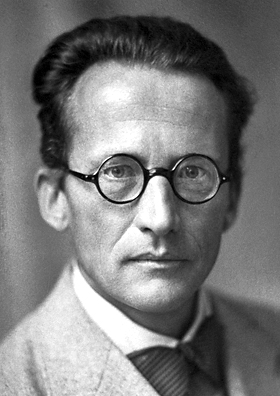
\includegraphics[width=\linewidth]{images/book3/schrodinger.jpg}
\end{minipage}\hfill
\begin{minipage}[t]{0.69\linewidth}\vspace{0pt}
{\small Erwin Schr\"odinger, who in 1926 wrote the wave equation whose
solutions for the hydrogen atom are the orbitals of this chapter, and recovered
from them the energy levels that Bohr had postulated. He shared the Nobel
Prize in Physics in 1933. (Photograph: Nobel Foundation, public domain,
Wikimedia Commons.)}
\end{minipage}
\end{omfigure}

\section{The radial part}

The probability of finding the electron between the spheres of radii $r$ and $r +
dr$ is $|\psi|^2$ integrated over the shell of volume $4\pi r^2\,dr$; for any
orbital, once the angles are integrated out, it is $r^2R^2\,dr$.

\begin{definition}[Radial distribution]\label{def:b2:atomic-orbitals:radial-distribution}
The \emph{radial distribution function}\index{radial distribution function} of
an orbital is $P(r) = r^2R_{nl}(r)^2$: $P(r)\,dr$ is the probability that the
electron lies between $r$ and $r + dr$ from the nucleus. The \emph{most probable
radius}\index{most probable radius} is the value of $r$ at its largest maximum.
\end{definition}

\begin{proposition}[Normalisation of 1s]\label{prop:b2:atomic-orbitals:normalised}
$\int_0^\infty P_{1s}(r)\,dr = 1$.
\end{proposition}

\begin{proof}
With $Z = 1$ and $r$ in units of $a_0$, $P_{1s} = 4r^2\mathrm e^{-2r}$. By parts twice,
$\int_0^\infty r^2\mathrm e^{-2r}\,dr = \frac22\int_0^\infty r\,\mathrm e^{-2r}\,dr =
\frac12\int_0^\infty\mathrm e^{-2r}\,dr = \frac14$, and $4 \times \frac14 = 1$.
\end{proof}

\begin{proposition}[Most probable radius]\label{prop:b2:atomic-orbitals:most-probable}
For the 1s orbital the \omterm{def:b2:atomic-orbitals:radial-distribution}{most probable radius} is $a_0/Z$. For an orbital with $l =
n - 1$ (1s, 2p, 3d, \dots), it is $n^2a_0/Z$.
\end{proposition}

\begin{proof}
For $l = n - 1$ the \omterm{def:b2:atomic-orbitals:radial-angular}{radial part} has no node: $R \propto \rho^{n-1}\mathrm e^{-\rho/n}$,
so $P \propto \rho^{2n}\mathrm e^{-2\rho/n}$ and $d\ln P/d\rho = 2n/\rho - 2/n$, zero
for $\rho = n^2$, that is $r = n^2a_0/Z$. With $n = 1$, $r = a_0/Z$.
\end{proof}

\begin{proposition}[Mean radius of 1s]\label{prop:b2:atomic-orbitals:mean-radius}
The mean distance of a 1s electron from the nucleus is $\langle r\rangle = 3a_0/(2Z)$,
larger than its \omterm{def:b2:atomic-orbitals:radial-distribution}{most probable radius}.
\end{proposition}

\begin{proof}
With $Z = 1$: $\langle r\rangle = \int_0^\infty r\,P(r)\,dr = 4\int_0^\infty r^3\mathrm e^{-2r}
\,dr = 4 \times 3!/2^4 = 3/2$. The distribution has a long tail at large $r$,
which pulls the mean beyond the maximum.
\end{proof}

\begin{definition}[Nodes]\label{def:b2:atomic-orbitals:node}
A \emph{nodal surface}\index{nodal surface} of an orbital is a surface on which
the \omterm{def:b2:atomic-orbitals:wavefunction}{wavefunction} is zero and changes sign. It is a \emph{radial node}\index{radial
node} (a sphere) when the \omterm{def:b2:atomic-orbitals:radial-angular}{radial part} vanishes, an \emph{angular
node}\index{angular node} (a plane or a cone through the nucleus) when the \omterm{def:b2:atomic-orbitals:radial-angular}{angular
part} does.
\end{definition}

\begin{proposition}[Counting nodes]\label{prop:b2:atomic-orbitals:nodes}
An orbital $(n, l)$ has $n - l - 1$ \omterm{def:b2:atomic-orbitals:node}{radial nodes} and $l$ \omterm{def:b2:atomic-orbitals:node}{angular nodes}, $n - 1$ in
all.
\end{proposition}

\begin{proof}
On the functions of \cref{thm:b2:atomic-orbitals:hydrogen}: $R_{2s}$ vanishes at
$\rho = 2$, $R_{3s}$ at the two roots of $2\rho^2 - 18\rho + 27$ ($\rho = 1.90$ and $7.10$),
$R_{3p}$ at $\rho = 6$; $R_{1s}$, $R_{2p}$, $R_{3d}$ do not vanish. The \omterm{def:b2:atomic-orbitals:radial-angular}{angular part}
of a p orbital vanishes on one plane ($z = 0$ for $p_z$), that of a d orbital on two
planes or, for $d_{z^2}$, on a cone. The general case is admitted.
\end{proof}

\begin{omfigure}
\begin{tikzpicture}
\begin{axis}[width=0.55\linewidth, height=6cm, xmin=0, xmax=24, ymin=0, ymax=0.58,
  axis x line=bottom, axis y line=left, xlabel={$r/a_0$}, ylabel={$P(r)$},
  tick label style={font=\small}, label style={font=\small}, title={\small radial distributions, $Z = 1$}]
\addplot[omThm, thick] table[x=r, y=s1] {figdata/out/bachelor-2-atomic-orbitals-a.dat};
\addplot[omDef, thick] table[x=r, y=s2] {figdata/out/bachelor-2-atomic-orbitals-a.dat};
\addplot[omDef, thick, dashed] table[x=r, y=p2] {figdata/out/bachelor-2-atomic-orbitals-a.dat};
\addplot[omProp, thick] table[x=r, y=s3] {figdata/out/bachelor-2-atomic-orbitals-a.dat};
\addplot[omProp, thick, dashed] table[x=r, y=p3] {figdata/out/bachelor-2-atomic-orbitals-a.dat};
\addplot[omProp, thick, dotted] table[x=r, y=d3] {figdata/out/bachelor-2-atomic-orbitals-a.dat};
\node[font=\scriptsize, omThm, anchor=west] at (axis cs:1.4,0.53) {1s};
\node[font=\scriptsize, omDef, anchor=south] at (axis cs:4.0,0.215) {2p};
\node[font=\scriptsize, omDef, anchor=south west] at (axis cs:6.4,0.17) {2s};
\node[font=\scriptsize, omProp, anchor=south] at (axis cs:10.5,0.12) {3d};
\node[font=\scriptsize, omProp, anchor=west] at (axis cs:17,0.085) {3s, 3p};
\end{axis}
\end{tikzpicture}\hfill
\begin{tikzpicture}
\begin{axis}[width=0.42\linewidth, height=6cm, xmin=0, xmax=20, ymin=-0.12, ymax=0.75,
  axis x line=middle, axis y line=left, xlabel={$r/a_0$}, ylabel={$R$},
  tick label style={font=\small}, label style={font=\small}, title={\small radial parts}]
\addplot[omDef, thick] table[x=r, y=R2s] {figdata/out/bachelor-2-atomic-orbitals-b.dat};
\addplot[omProp, thick] table[x=r, y=R3s] {figdata/out/bachelor-2-atomic-orbitals-b.dat};
\node[font=\scriptsize, omDef, anchor=west] at (axis cs:0.4,0.62) {$R_{2s}$};
\node[font=\scriptsize, omProp, anchor=west] at (axis cs:0.6,0.30) {$R_{3s}$};
\node[font=\scriptsize, anchor=south west] at (axis cs:3,0.15) {node};
\draw[thin, ->] (axis cs:3,0.15) -- (axis cs:2.05,0.01);
\end{axis}
\end{tikzpicture}

{\small Left: radial distributions $P(r) = r^2R^2$ of the orbitals of hydrogen up
to $n = 3$; the larger $n$, the farther the electron, and the s orbitals have
small inner maxima (penetration). Right: $R_{2s}$ and $R_{3s}$ change sign at their
\omterm{def:b2:atomic-orbitals:node}{radial nodes} ($r = 2a_0$; $1.90a_0$ and $7.10a_0$).}
\end{omfigure}

\begin{omfigure}
\begin{tikzpicture}
\begin{axis}[scale only axis, width=0.32\linewidth, height=0.32\linewidth,
  xmin=-6, xmax=6, ymin=-6, ymax=6, axis lines=none, title={\small 1s}]
\addplot[only marks, mark=*, mark size=0.25pt, omDef] table[x=x, y=y] {figdata/out/bachelor-2-atomic-orbitals-c-1s.dat};
\end{axis}
\end{tikzpicture}\hspace{0.12\linewidth}%
\begin{tikzpicture}
\begin{axis}[scale only axis, width=0.32\linewidth, height=0.32\linewidth,
  xmin=-14, xmax=14, ymin=-14, ymax=14, axis lines=none, title={\small 2s}]
\addplot[only marks, mark=*, mark size=0.25pt, omDef] table[x=x, y=y] {figdata/out/bachelor-2-atomic-orbitals-c-2s.dat};
\draw[densely dashed, omThm] (axis cs:0,0) circle[radius=2];
\end{axis}
\end{tikzpicture}

{\small Dot-density pictures of the 1s and 2s orbitals of hydrogen in a plane
through the nucleus: the density of dots follows $|\psi|^2$ (deterministic
sampling). The 2s cloud has an empty ring, the \omterm{def:b2:atomic-orbitals:node}{radial node} at $2a_0$ (dashed);
the frames are 12 and 28 $a_0$ wide.}
\end{omfigure}

\section{The angular part}

The \omterm{def:b2:atomic-orbitals:radial-angular}{angular part} fixes the shape. An s orbital is spherical; a p orbital has two
lobes of opposite signs along its axis, separated by a nodal plane; a d orbital has
four lobes of alternating signs (or, for $d_{z^2}$, two lobes and a ring). The sign
of a lobe has no physical meaning by itself --- $\psi$ and $-\psi$ describe the same
state --- but the relative signs of two orbitals decide, in the next chapter,
whether they combine into a bond.

\begin{omfigure}
\begin{tikzpicture}[font=\small]
  \pic at (0,0) {oms={1}};
  \node[below] at (0,-0.75) {s};
  \pic at (2.0,0) {omp={1}{0}};
  \draw[->, black!55, thin] (1.0,0) -- (3.0,0) node[right, font=\tiny] {$x$};
  \node[below] at (2.0,-0.75) {$\mathrm p_x$};
  \pic at (4.2,0) {omp={1}{90}};
  \draw[->, black!55, thin] (4.2,-0.95) -- (4.2,0.95) node[above, font=\tiny] {$z$};
  \node[below] at (4.75,-0.75) {$\mathrm p_z$};
  \pic at (6.6,0) {omdxy}; \node[below] at (6.6,-1.0) {$\mathrm d_{xy}$};
  \pic at (9.0,0) {omdx2y2}; \node[below] at (9.0,-1.0) {$\mathrm d_{x^2-y^2}$};
  \pic at (11.4,0) {omdz2}; \node[below] at (11.4,-1.0) {$\mathrm d_{z^2}$};
\end{tikzpicture}

{\small Real atomic orbitals, schematic: the lobes show the regions where $|\psi|$
is large, coloured by the sign of $\psi$ (blue positive, orange negative). The
$\mathrm d_{xz}$ and $\mathrm d_{yz}$ orbitals have the shape of $\mathrm d_{xy}$ in
the planes their names give.}
\end{omfigure}

\begin{method}[Sketching an orbital from its quantum numbers]\label{met:b2:atomic-orbitals:draw-orbital}
\begin{enumerate}
  \item From $l$, the shape: s (sphere), p (two lobes), d (four lobes, or two
        lobes and a ring for $d_{z^2}$); from the subscript, the orientation.
  \item Count the $l$ \omterm{def:b2:atomic-orbitals:node}{angular nodes} (planes through the nucleus) and give
        adjacent lobes opposite signs.
  \item Count the $n - l - 1$ \omterm{def:b2:atomic-orbitals:node}{radial nodes}: inner shells of opposite sign inside
        the main lobes (usually left out of sketches).
  \item Scale with $n^2a_0/Z$: higher $n$, larger orbital; larger $Z$, smaller.
\end{enumerate}
\end{method}

\section{Many-electron atoms}

In an atom with several electrons, each electron feels the nucleus screened by
the others. The orbitals keep the shapes of the hydrogen ones, with an effective
charge $Z^*$ in place of $Z$, and the energy of a subshell now depends on $l$ as
well as on $n$: an s electron, whose radial distribution has inner maxima close to
the nucleus, is screened less than a p electron of the same shell, and a p less
than a d.

\begin{definition}[Slater's rules]\label{def:b2:atomic-orbitals:slater}
\emph{Slater's rules}\index{Slater's rules} estimate the effective nuclear charge
$Z^* = Z - \sigma$ felt by an electron. The electrons are grouped as
(1s) (2s, 2p) (3s, 3p) (3d) (4s, 4p) (4d) (4f) (5s, 5p) \dots; the screening
constant $\sigma$ of an electron is the sum of the contributions of the other
electrons: 0.35 for each other electron of the same group (0.30 within 1s);
for an s or p electron, 0.85 for each electron of the shell $n - 1$ and 1.00 for
each electron of lower shells; for a d or f electron, 1.00 for every electron
of the groups below its own. Groups above contribute nothing.
\end{definition}

\begin{omfigure}
\small
\renewcommand{\arraystretch}{1.2}
\begin{tabular}{l|ccccc}
electron studied & same group & shell $n - 1$ & lower shells & groups above \\ \hline
1s & 0.30 & --- & --- & 0 \\
$n$s, $n$p & 0.35 & 0.85 & 1.00 & 0 \\
$n$d, $n$f & 0.35 & 1.00 & 1.00 & 0 \\
\end{tabular}

\smallskip
{\small Slater's screening constants, per screening electron. The effective
principal quantum numbers are $n^* = 1, 2, 3, 3.7, 4.0, 4.2$ for $n = 1$ to 6.}
\end{omfigure}

\begin{method}[Computing an effective charge]\label{met:b2:atomic-orbitals:slater}
\begin{enumerate}
  \item Write the configuration in Slater's groups, in order of $n$, with s and p
        together and d and f apart.
  \item Pick the electron; add 0.35 for each other electron of its group.
  \item Add 0.85 (s or p electron) or 1.00 (d or f) per electron of the shell just
        below, and 1.00 per electron deeper.
  \item $Z^* = Z - \sigma$.
\end{enumerate}
\end{method}

\begin{definition}[Orbital energy and radius]\label{def:b2:atomic-orbitals:orbital-energy}
In Slater's model, the \emph{orbital energy}\index{orbital energy} of an electron
of effective charge $Z^*$ and effective principal quantum number $n^*$ is
$\varepsilon = -E_RZ^{*2}/n^{*2}$, and its \emph{orbital radius}\index{orbital radius}
is $n^{*2}a_0/Z^*$, the \omterm{def:b2:atomic-orbitals:radial-distribution}{most probable radius} of a hydrogen-like orbital of charge
$Z^*$.
\end{definition}

\begin{proposition}[Slater energies]\label{prop:b2:atomic-orbitals:slater-energy}
The energy of a group of $k$ electrons of effective charge $Z^*$ is approximately
$k\varepsilon = -kE_RZ^{*2}/n^{*2}$, and the total electronic energy of the atom
is the sum over its groups.
\end{proposition}

\admitted

\begin{example}[Iron: 4s or 3d first?]\label{ex:b2:atomic-orbitals:iron}
Iron is $[\ce{Ar}]\,3\mathrm d^6\,4\mathrm s^2$. A 4s electron: $\sigma = 0.35 + 14
\times 0.85 + 10 \times 1.00 = 22.25$, $Z^* = 3.75$, $\varepsilon = -13.6 \times
3.75^2/3.7^2 = \qty{-14.0}{eV}$. A 3d electron: $\sigma = 5 \times 0.35 + 18 \times 1.00 =
19.75$, $Z^* = 6.25$, $\varepsilon = -13.6 \times 6.25^2/9 = \qty{-59}{eV}$. The 3d
electrons are much more tightly bound: although 4s is filled first in the
building-up order, it is a 4s electron that leaves when iron is ionised, and the
iron(II) ion is $[\ce{Ar}]\,3\mathrm d^6$.
\end{example}

\section{Using orbital energies and sizes}

\begin{proposition}[Ionisation energy from Slater energies]\label{prop:b2:atomic-orbitals:ionisation}
In Slater's model, the first ionisation energy of an atom is the difference
between the total energies of the ion and of the atom, computed group by group
with the effective charges of each.
\end{proposition}

\begin{proof}
The ionisation energy is $E(\text{ion}) - E(\text{atom})$; by
\cref{prop:b2:atomic-orbitals:slater-energy}, both are sums of group energies, and
only the group losing the electron changes (inner groups are not screened by
outer electrons).
\end{proof}

\begin{example}[Carbon]\label{ex:b2:atomic-orbitals:carbon}
Carbon, (2s, 2p)$^4$: $Z^* = 6 - 2 \times 0.85 - 3 \times 0.35 = 3.25$; the group energy is
$4 \times (-13.6 \times 3.25^2/4) = \qty{-143.6}{eV}$. The ion \ce{C+}, (2s, 2p)$^3$: $Z^* =
3.60$, $3 \times (-13.6 \times 3.60^2/4) = \qty{-132.2}{eV}$. The ionisation energy is
\qty{11.5}{eV}, against \qty{11.26}{eV} measured.
% ledger: ie:C, const:RyhcEV
\end{example}

\begin{omfigure}
\begin{tikzpicture}
\begin{axis}[width=0.47\linewidth, height=5.4cm, xmin=0.5, xmax=8.5, ymin=0, ymax=6.5,
  axis x line=bottom, axis y line=left, xtick={1,2,3,4,5,6,7,8},
  xticklabels={Li,Be,B,C,N,O,F,Ne}, tick label style={font=\small},
  label style={font=\small}, title={\small period 2}]
\addplot[omThm, thick, mark=*, mark size=1.3pt] table[x=k, y=zs] {figdata/out/bachelor-2-atomic-orbitals-d-period.dat};
\addplot[omDef, thick, mark=square*, mark size=1.3pt] table[x=k, y=r] {figdata/out/bachelor-2-atomic-orbitals-d-period.dat};
\node[font=\scriptsize, omThm, anchor=south east] at (axis cs:7.8,5.3) {$Z^*$};
\node[font=\scriptsize, omDef, anchor=south west] at (axis cs:1.2,3.1) {radius ($a_0$)};
\end{axis}
\end{tikzpicture}\hfill
\begin{tikzpicture}
\begin{axis}[width=0.47\linewidth, height=5.4cm, xmin=1.5, xmax=6.5, ymin=0, ymax=9,
  axis x line=bottom, axis y line=left, xtick={2,3,4,5,6},
  xticklabels={Li,Na,K,Rb,Cs}, tick label style={font=\small},
  label style={font=\small}, title={\small group 1}]
\addplot[omThm, thick, mark=*, mark size=1.3pt] table[x=n, y=zs] {figdata/out/bachelor-2-atomic-orbitals-d-group.dat};
\addplot[omDef, thick, mark=square*, mark size=1.3pt] table[x=n, y=r] {figdata/out/bachelor-2-atomic-orbitals-d-group.dat};
\node[font=\scriptsize, omThm, anchor=north] at (axis cs:4,2.0) {$Z^*$};
\node[font=\scriptsize, omDef, anchor=west] at (axis cs:2.1,5.4) {radius ($a_0$)};
\end{axis}
\end{tikzpicture}

{\small Slater's effective charge of the valence electron and \omterm{def:b2:atomic-orbitals:orbital-energy}{orbital radius}
$n^{*2}a_0/Z^*$. Along period 2, $Z^*$ grows by 0.65 per element and the atoms
shrink; down group 1, $Z^*$ stays at 1.30 then 2.20 while $n^*$ grows, and the atoms
swell.}
\end{omfigure}

The model reproduces the trends of the Year 1 volume. Along a period, each
added proton is screened by only 0.35 of the electron added with it: $Z^*$ rises,
the outer orbital contracts and binds more strongly. Down a group, $Z^*$ hardly
changes while the outer shell moves out: atoms grow and their ionisation energies
fall. Sodium, with $Z^* = 2.20$ for its 3s electron, has an \omterm{def:b2:atomic-orbitals:orbital-energy}{orbital radius} of
$9/2.2 = 4.1a_0$; chlorine, with $Z^* = 6.10$ for a 3p electron, $9/6.1 = 1.5a_0$.

\section{Exercises}

\begin{exercise}[$\star$]\label{exo:b2:atomic-orbitals:1}
Give the quantum numbers $n$ and $l$, the number of \omterm{def:b2:atomic-orbitals:node}{radial nodes} and of \omterm{def:b2:atomic-orbitals:node}{angular
nodes} of a 3p and of a 4d orbital.
\end{exercise}

\begin{exercise}[$\star$]\label{exo:b2:atomic-orbitals:2}
Show from $R_{2p}$ that the \omterm{def:b2:atomic-orbitals:radial-distribution}{most probable radius} of a 2p electron of hydrogen is
$4a_0$, and give it in picometres.
\end{exercise}

\begin{exercise}[$\star$]\label{exo:b2:atomic-orbitals:3}
Compute the probability of finding the 1s electron of hydrogen closer to the
nucleus than $a_0$.
\end{exercise}

\begin{exercise}[$\star$]\label{exo:b2:atomic-orbitals:4}
Sketch the $3\mathrm d_{xy}$ orbital: lobes, signs, nodal planes. How many \omterm{def:b2:atomic-orbitals:node}{radial
nodes} does it have?
\end{exercise}

\begin{exercise}[$\star\star$]\label{exo:b2:atomic-orbitals:5}
Compute Slater's effective charge for a 2p electron of oxygen and the \omterm{def:b2:atomic-orbitals:orbital-energy}{orbital
radius} it gives.
\end{exercise}

\begin{exercise}[$\star\star$]\label{exo:b2:atomic-orbitals:6}
Using the example of iron, explain why the configuration of \ce{Fe^3+} is
$[\ce{Ar}]\,3\mathrm d^5$ and not $[\ce{Ar}]\,3\mathrm d^3 4\mathrm s^2$.
\end{exercise}

\begin{exercise}[$\star\star$]\label{exo:b2:atomic-orbitals:7}
Estimate by \omterm{def:b2:atomic-orbitals:slater}{Slater's rules} the first ionisation energies of lithium and sodium,
and compare with the measured 5.39 and \qty{5.14}{eV}. Comment.
\end{exercise}

\begin{exercise}[$\star\star$]\label{exo:b2:atomic-orbitals:8}
Compute $Z^*$ and the \omterm{def:b2:atomic-orbitals:orbital-energy}{orbital radius} of the outer electron of sodium and of
chlorine, and explain why the sodium atom is the larger.
\end{exercise}

\begin{exercise}[$\star\star$]\label{exo:b2:atomic-orbitals:9}
Show that the 1s and 2s orbitals of hydrogen are orthogonal,
$\int\psi_{1s}\psi_{2s}\,dV = 0$.
\end{exercise}

\begin{exercise}[$\star\star\star$]\label{exo:b2:atomic-orbitals:10}
Write $R_{2p} = N\rho\,\mathrm e^{-\rho/2}$ and find the constant $N$ that normalises it
($Z = 1$, $r$ in units of $a_0$).
\end{exercise}

\begin{exercise}[$\star\star\star$]\label{exo:b2:atomic-orbitals:11}
Compare the mean radius and the \omterm{def:b2:atomic-orbitals:radial-distribution}{most probable radius} of a 1s electron, and
explain from the shape of $P(r)$ why they differ.
\end{exercise}

\begin{exercise}[$\star\star\star$]\label{exo:b2:atomic-orbitals:12}
Find the \omterm{def:b2:atomic-orbitals:node}{nodal surface} of the $\mathrm p_z$ orbital and show that $\psi_{2p_z}$
changes sign across it. What is the \omterm{def:b2:atomic-orbitals:wavefunction}{probability density} on that surface?
\end{exercise}

\section{Problem: Where Is the Electron?}

\begin{problem}[{Weekend problem --- the 1s orbital of hydrogen and its radii,
the probability of finding the electron beyond a given distance, the nodes and
maxima of 2s and 2p, and Slater's estimate of the ionisation energies of carbon,
nitrogen and oxygen}]
\label{pb:b2:atomic-orbitals:1}
Data: $a_0 = \qty{52.9}{pm}$; $E_R = \qty{13.6}{eV}$; measured first ionisation
energies (\unit{eV}): C 11.26, N 14.53, O 13.62. $\psi_{1s} = \pi^{-1/2}a_0^{-3/2}\,
\mathrm e^{-r/a_0}$.
% ledger: const:a0, const:RyhcEV, ie:C, ie:N, ie:O

\medskip
\noindent\textbf{Part I --- The 1s orbital.}
\begin{enumerate}
  \item Check that $\psi_{1s}$ is normalised, using $dV = 4\pi r^2\,dr$.
  \item Write the \omterm{def:b2:atomic-orbitals:radial-distribution}{radial distribution function} $P(r)$.
  \item Find the \omterm{def:b2:atomic-orbitals:radial-distribution}{most probable radius}.
  \item Compute the mean radius.
  \item Why is the mean larger than the \omterm{def:b2:atomic-orbitals:radial-distribution}{most probable radius}?
  \item The \omterm{def:b2:atomic-orbitals:wavefunction}{probability density} is largest at the nucleus, yet $P(0) = 0$.
        Explain.
  \item Give the \omterm{def:b2:atomic-orbitals:radial-distribution}{most probable radius} in picometres.
\end{enumerate}

\medskip
\noindent\textbf{Part II --- Beyond a radius.}
\begin{enumerate}[resume]
  \item Show that the probability of finding the electron farther than $r_0 =
        xa_0$ is $\mathrm e^{-2x}(1 + 2x + 2x^2)$.
  \item Compute it for $r_0 = a_0$.
  \item Compute it for $r_0 = 2a_0$.
  \item Find by trial the radius of the sphere that contains the electron with a
        probability of 0.90.
  \item In what sense does an atom have no edge, and in what sense a size?
\end{enumerate}

\medskip
\noindent\textbf{Part III --- 2s and 2p.}
\begin{enumerate}[resume]
  \item Give the nodes of 2s and of 2p (number, kind, position).
  \item Where does $R_{2s}$ change sign?
  \item Find the \omterm{def:b2:atomic-orbitals:radial-distribution}{most probable radius} of 2p.
  \item Find the two maxima of $P_{2s} \propto r^2(2 - r)^2\mathrm e^{-r}$ ($r$ in units of
        $a_0$).
  \item Which of 2s and 2p has electron density closer to the nucleus? What does
        it imply in a many-electron atom?
  \item How do these radii change for the hydrogen-like ion \ce{C^5+}?
\end{enumerate}

\medskip
\noindent\textbf{Part IV --- Carbon, nitrogen, oxygen.}
\begin{enumerate}[resume]
  \item Compute Slater's $Z^*$ of a 2p electron in C, N and O.
  \item Compute the corresponding orbital energies.
  \item Estimate the first ionisation energy of carbon as a difference of group
        energies.
  \item Same for nitrogen.
  \item Same for oxygen, and compare the three with the measured values.
  \item Which feature of the measured values does the model miss, and why?
  \item State the probability of finding the 1s electron of hydrogen farther
        than $2a_0$.
\end{enumerate}
\end{problem}
